\newpage
\section*{Assignment 10b: Co-creation} 
\noindent
\makebox[\textwidth]{\includegraphics{table.pdf}}
% \includepdf[pages=-]{/table.pdf}

% \subsection*{Social practises}
% \subsubsection*{Users}
% Drivers will enter autonomous vehicles and merely input the desired destination. The vehicle when then proceed to the desired destination fully automated.
% The autonomous vehicles can be configured with different interiors to accommodate different situations, like a small office desk space for working, multiple seats to accommodate multiple people or even a mini cinema for entertainment during travels. 
% The users would find, modify and change the interior configuration to needs etc.

% \subsubsection*{Designers}
% Designers will explore the ideas of users and optimize and create parts to accommodate interior designs. Further optimizations and development will also be a practice of the designers.


% \subsection*{Expectations}
% \subsubsection*{Users}
% Users expect the continued access and operation of the technology. Some might even expect a more efficient system, perhaps even water or airborne.

% \subsubsection*{Designers}
% Designers expect everyone to one day uses the technology, and this would open a new avenue of transport infrastructure.


% \subsection*{Infrastructures}
% \subsubsection*{Designers}
% Servers for software and updates, perhaps even servers for other types of digital control with autonomous vehicles, manufacturing facilities, power facilities and viable compatible roads for the vehicles.

% \subsubsection*{Users}
% Storage solutions, like garages and parking spots, perhaps with the addition of charging stations would be necessary to facilitate autonomous vehicles.

% \subsection*{Possibilities and limitations}
% \subsubsection*{Designers}


% \subsubsection*{Users}
% Users could think that space is limited, by the nature of having to operate on current road infrastructures.

